\begin{figure*}[h]
\centering
\resizebox{\textwidth}{!}{%
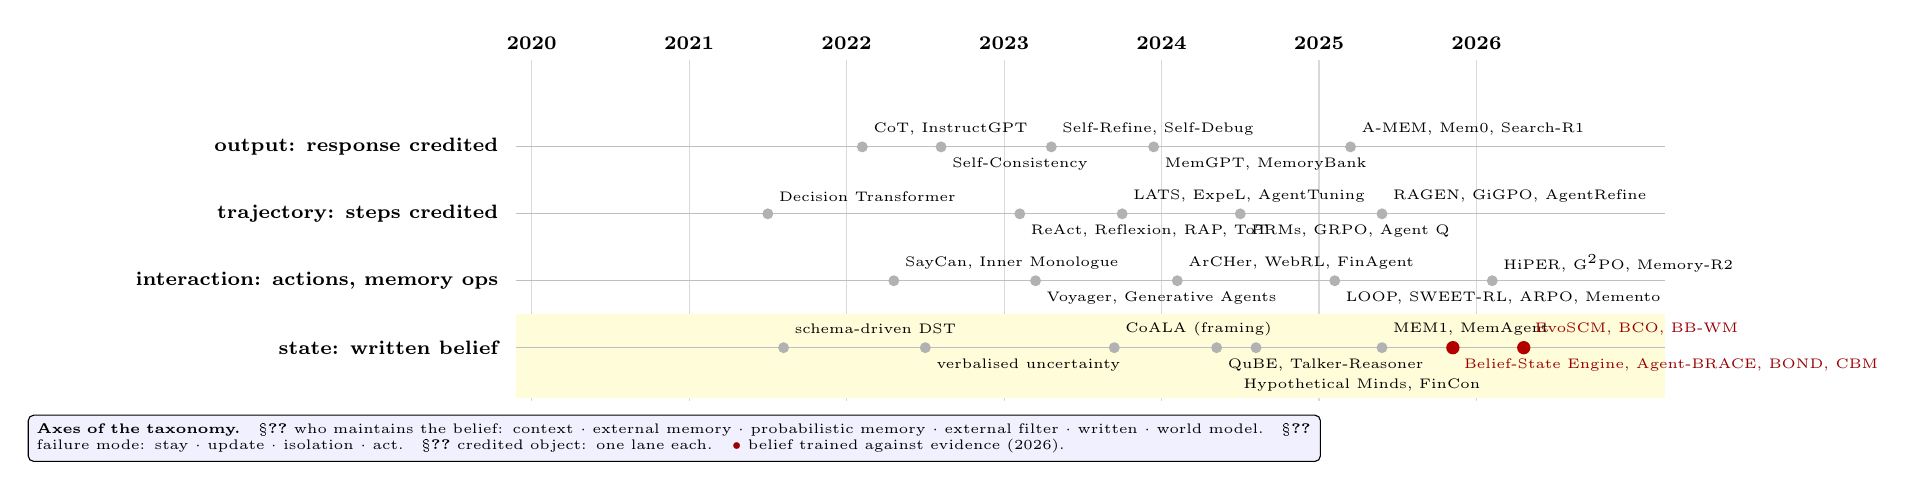
\begin{tikzpicture}[x=2.0cm, y=0.85cm, font=\scriptsize,
  lane/.style={font=\scriptsize\bfseries, anchor=east},
  pt/.style={circle, fill=gray!60, inner sep=1.4pt},
  ptS/.style={circle, fill=red!70!black, inner sep=1.7pt},
  lbl/.style={font=\tiny, anchor=west, inner sep=1pt},
  lblS/.style={font=\tiny, anchor=west, inner sep=1pt, text=red!60!black}]
\foreach \yr/\x in {2020/0, 2021/1, 2022/2, 2023/3, 2024/4, 2025/5, 2026/6} {
  \node[font=\scriptsize\bfseries] at (\x,0.55) {\yr};
  \draw[gray!30] (\x,0.3) -- (\x,-4.8); }
\fill[yellow!15] (-0.1,-4.75) rectangle (7.2,-3.5);
\foreach \name/\y in {{\textbf{output}: response credited}/-1, {\textbf{trajectory}: steps credited}/-2, {\textbf{interaction}: actions, memory ops}/-3, {\textbf{state}: written belief}/-4}
  \node[lane] at (-0.15,\y) {\name};
\foreach \y in {-1,-2,-3,-4} \draw[gray!50] (-0.1,\y) -- (7.2,\y);
% output lane
\node[pt] at (2.1,-1) {}; \node[lbl] at (2.15,-0.74) {CoT, InstructGPT};
\node[pt] at (2.6,-1) {}; \node[lbl] at (2.65,-1.26) {Self-Consistency};
\node[pt] at (3.3,-1) {}; \node[lbl] at (3.35,-0.74) {Self-Refine, Self-Debug};
\node[pt] at (3.95,-1) {}; \node[lbl] at (4.0,-1.26) {MemGPT, MemoryBank};
\node[pt] at (5.2,-1) {}; \node[lbl] at (5.25,-0.74) {A-MEM, Mem0, Search-R1};
% trajectory lane
\node[pt] at (1.5,-2) {}; \node[lbl] at (1.55,-1.74) {Decision Transformer};
\node[pt] at (3.1,-2) {}; \node[lbl] at (3.15,-2.26) {ReAct, Reflexion, RAP, ToT};
\node[pt] at (3.75,-2) {}; \node[lbl] at (3.8,-1.74) {LATS, ExpeL, AgentTuning};
\node[pt] at (4.5,-2) {}; \node[lbl] at (4.55,-2.26) {PRMs, GRPO, Agent Q};
\node[pt] at (5.4,-2) {}; \node[lbl] at (5.45,-1.74) {RAGEN, GiGPO, AgentRefine};
% interaction lane
\node[pt] at (2.3,-3) {}; \node[lbl] at (2.35,-2.74) {SayCan, Inner Monologue};
\node[pt] at (3.2,-3) {}; \node[lbl] at (3.25,-3.26) {Voyager, Generative Agents};
\node[pt] at (4.1,-3) {}; \node[lbl] at (4.15,-2.74) {ArCHer, WebRL, FinAgent};
\node[pt] at (5.1,-3) {}; \node[lbl] at (5.15,-3.26) {LOOP, SWEET-RL, ARPO, Memento};
\node[pt] at (6.1,-3) {}; \node[lbl] at (6.15,-2.74) {HiPER, G$^2$PO, Memory-R2};
% state lane (three label rows)
\node[pt] at (1.6,-4) {}; \node[lbl] at (1.65,-3.72) {schema-driven DST};
\node[pt] at (2.5,-4) {}; \node[lbl] at (2.55,-4.26) {verbalised uncertainty};
\node[pt] at (3.7,-4) {}; \node[lbl] at (3.75,-3.72) {CoALA (framing)};
\node[pt] at (4.35,-4) {}; \node[lbl] at (4.4,-4.26) {QuBE, Talker-Reasoner};
\node[pt] at (4.6,-4) {}; \node[lbl] at (4.5,-4.56) {Hypothetical Minds, FinCon};
\node[pt] at (5.4,-4) {}; \node[lbl] at (5.45,-3.72) {MEM1, MemAgent};
\node[ptS] at (5.85,-4) {}; \node[lblS] at (5.9,-4.26) {Belief-State Engine, Agent-BRACE, BOND, CBM};
\node[ptS] at (6.3,-4) {}; \node[lblS] at (6.35,-3.72) {EvoSCM, BCO, BB-WM};
% legend
\node[draw, rounded corners=2pt, fill=blue!6, align=left, font=\tiny, anchor=north west, inner sep=3pt, text width=16.2cm] at (-3.2,-5.0) {%
\textbf{Axes of the taxonomy.}\quad
\S\ref{sec:representation} who maintains the belief: context $\cdot$ external memory $\cdot$ probabilistic memory $\cdot$ external filter $\cdot$ written $\cdot$ world model.\quad
\S\ref{sec:revision} failure mode: stay $\cdot$ update $\cdot$ isolation $\cdot$ act.\quad
\S\ref{sec:learning} credited object: one lane each.\quad
{\color{red!60!black}$\bullet$} belief trained against evidence (2026).};
\end{tikzpicture}}
\caption{Where credit has gone, 2020--2026. Lanes are credited objects; Table~\ref{tab:master} lists every screened system. Written beliefs exist from dialogue state tracking onward, but until 2026 they are credited by task outcome or not trained at all; the red points are the first to give the belief its own learning signal.}
\label{fig:timeline}
\end{figure*}
